% reducesymm/QFT/finiteBlog.tex
% $Author$ $Date$
% Predrag  switched to github.com               jul  8 2013

\section{Is QED finite? A blog}
\label{sect:finiteBlog}

\begin{description}

\item[2013-12-08  Predrag] to Piotr, Wanda and Andrea
(Piotr Czerski <piotr.czerski@ifj.edu.pl>,
 wanda.alberico@to.infn.it,
 andrea.prunotto@gmail.com):

I'm no fan of Feynman diagrams, and I'm always looking
for other ways to look at perturbative expansions. So just a little email
- if you have a new angle\rf{PrAlCz13} on subsets of diagrams which are gauge
invariant sets, I would be curious to learn how you look at that.

Just something to keep in mind :)

PS to Andrea: I realize you might rather forget this stuff (takes you a
decade to write a paper?) but at least I got a ringtone out of you. The
only problem is, I do not have a cell phone, so I do not know how to make
it ring. At least I'm more technologically savvy than
\HREF{http://www.theguardian.com/science/2013/dec/06/peter-higgs-boson-academic-system?CMP=twt_gu}
{Peter Higgs}.

\item[2013-12-10  \HREF{https://sites.google.com/site/andreaprunotto/} {Andrea}]
Sorry for late reply (well, we're used to longer gaps). Yes! I actually
took 10 years to write this paper out of my master thesis, but I have
some excuses: I did my PhD in Biochemistry (Z\"urich) and now I work on
genetics (Lausanne). This summer my ``old'' professor Wanda found my work
in a drawer and then contacted me, telling me that it would be a good
idea to publish it.

About your request: I'm really interested in seeing if the rooted-map
approach to Feynman diagrams can address the problem you've risen. But I
have no idea what the ''subsets of diagrams which are gauge invariant
sets'' are. I've checked a bit on the web but I'm sure you can give me
better indications (the works I found were too technical: I need to know
the basis of the problem). Can you send me some specific link at freshman
level, in particular where I can see the geometry of these subclasses of
diagrams?

\item[2013-12-11  Predrag]
Why Google when you can click on the link in my email?

    ... I'm no fan of Feynman diagrams (my rant is
\HREF{http://www.cns.gatech.edu/~predrag/papers/preprints.html\#FiniteFieldTheo}
{here}) ... The article defines the gauge invariant sets.

\item[2016-02-08  Predrag]
Prunotto, Alberico and Czerski
{\em Feynman Diagrams and Rooted Maps}\rf{PrAlCz13}
has been submitted to the European Physical Journal A as manuscript ID EPJA-103480.
I have been asked to referee it, but have declined - too busy. They write: ``
The  Rooted Maps Theory, a branch of the Theory of Homology, is shown to be
a powerful tool for investigating  the topological properties of Feynman
diagrams, related to the single particle propagator in the quantum many-body
systems. The numerical correspondence between the number of this class of
Feynman diagrams as a function of perturbative order and the number of rooted
maps as a function of the number of edges is studied. A graphical procedure to
associate Feynman diagrams and rooted maps is then stated. Finally, starting
from rooted maps principles, an original definition of the genus of a
Feynman diagram, which totally differs from the usual one, is given.
''

\item[2016-12-10 Predrag]
Penante\rf{Penante16} {{On-shell methods for off-shell quantities in N=4
Super Yang-Mills: from scattering amplitudes to form factors and the
dilatation operator}} has an up-to-date review of on-shell methods.

\item[2016-12-26 Predrag] Read
Cruz-Santiago, Kotko and Sta{\'s}to\rf{CrKoSt15}
{\em Scattering amplitudes in the light-front formalism}:
``The idea is to divide the process into appropriate gauge invariant
components. It turns out that the gauge invariant subsets are invariant
under cyclic permutations of the external gluons. This decomposition was
proposed in works of [58–61] for the tree level amplitudes. A thorough
analysis of the relation between color structures and gauge invariance
was done in \refref{NPB81}. The color decomposition principle was
extended beyond the tree level to loop amplitudes in [63].''

Should also read Dixon\rf{Dixon96}
{\em Calculating scattering amplitudes efficiently}.

\item[2017-03-15 Predrag] Read
Dunne and Krasnansky\rf{DunKra06} {\em ``Background field
integration-by-parts'' and the connection between one-loop and two-loop
{Heisenberg-Euler} effective actions}: ``
We develop integration-by-parts rules for diagrams involving massive
scalar propagators in a constant background electromagnetic field, and
use these to show that there is a simple diagrammatic interpretation of
mass renormalization in the two-loop scalar QED Heisenberg-Euler
effective action for a general constant background field. This explains
why the square of a one-loop term appears in the renormalized two-loop
Heisenberg-Euler effective action. No integrals need be evaluated, and
the explicit form of the background field propagators is not needed. This
dramatically simplifies the computation of the renormalized two-loop
effective action for scalar QED, and generalizes a previous result
obtained for self-dual background fields.
''

\item[2017-05-23 Predrag]
M. G. Schmidt and C. Schubert\rf{SchSch96},
{\em Multiloop calculations in the string-inspired formalism: the single
spinor-loop in QED}, \arXiv{hep-th/9410100}.

\item[2017-05-23 Predrag]
Christian Schubert\rf{Schubert01}
{\em Perturbative quantum field theory in the string-inspired formalism},
\arXiv{hep-th/0101036}:

\item[2017-03-15 Predrag] Read
Huet, McKeon, and Schubert\rf{HuMcSc10}
{\em {Euler-Heisenberg} lagrangians and asymptotic analysis in 1+1 {QED. Part I: Two}-loop}
(no GaTech online access, have not checked arXiv):``
We continue an effort to obtain information on the QED perturbation
series at high loop orders, and particularly on the issue of large
cancellations inside gauge invariant classes of graphs, using the example
of the l --- loop N --- photon amplitudes in the limit of large photon
numbers and low photon energies. As was previously shown, high-order
information on these amplitudes can be obtained from a nonperturbative
formula, due to Affleck et al., for the imaginary part of the QED
effective lagrangian in a constant field. The procedure uses Borel
analysis and leads, under some plausible assumptions, to a number of
nontrivial predictions already at the three-loop level. Their direct
verification would require a calculation of this `Euler-Heisenberg
lagrangian' at three-loops, which seems presently out of reach. Motivated
by previous work by Dunne and Krasnansky\rf{DunKra06} on Euler-Heisenberg
lagrangians in various dimensions, in the present work we initiate a new
line of attack on this problem by deriving and proving the analogous
predictions in the simpler setting of 1+1 dimensional QED. In the first
part of this series, we obtain a generalization of the formula of Affleck
et al. to this case, and show that, for both Scalar and Spinor QED, it
correctly predicts the leading asymptotic behaviour of the weak field
expansion coefficients of the two loop Euler-Heisenberg lagrangians.

\item[2017-05-23 Predrag]
Bastianelli, Huet, Schubert, Thakur and Weber\rf{BHSTW14}
{\em Integral representations combining ladders and crossed-ladders}
write:

``worldline formalism'' has been studied by many authors, and extended to
other field theories (see Schubert\rf{Schubert01} for an extensive
bibliography). One of the interesting aspects of this approach is that
often it combines into a single expression contributions from a large
number of Feynman diagrams. For example, in the QED case it generally
allows one to combine into one integral all contributions from Feynman
diagrams which can be identified by letting photon legs slide along
scalar/fermion loops or lines. At higher loop orders the summation will
generally involve topologically different diagrams;  as an example, we
show in \reffig{BHSTW143loopphotonprop} the ``quenched'' contributions to
the three-loop photon propagator.

\begin{figure}[h]
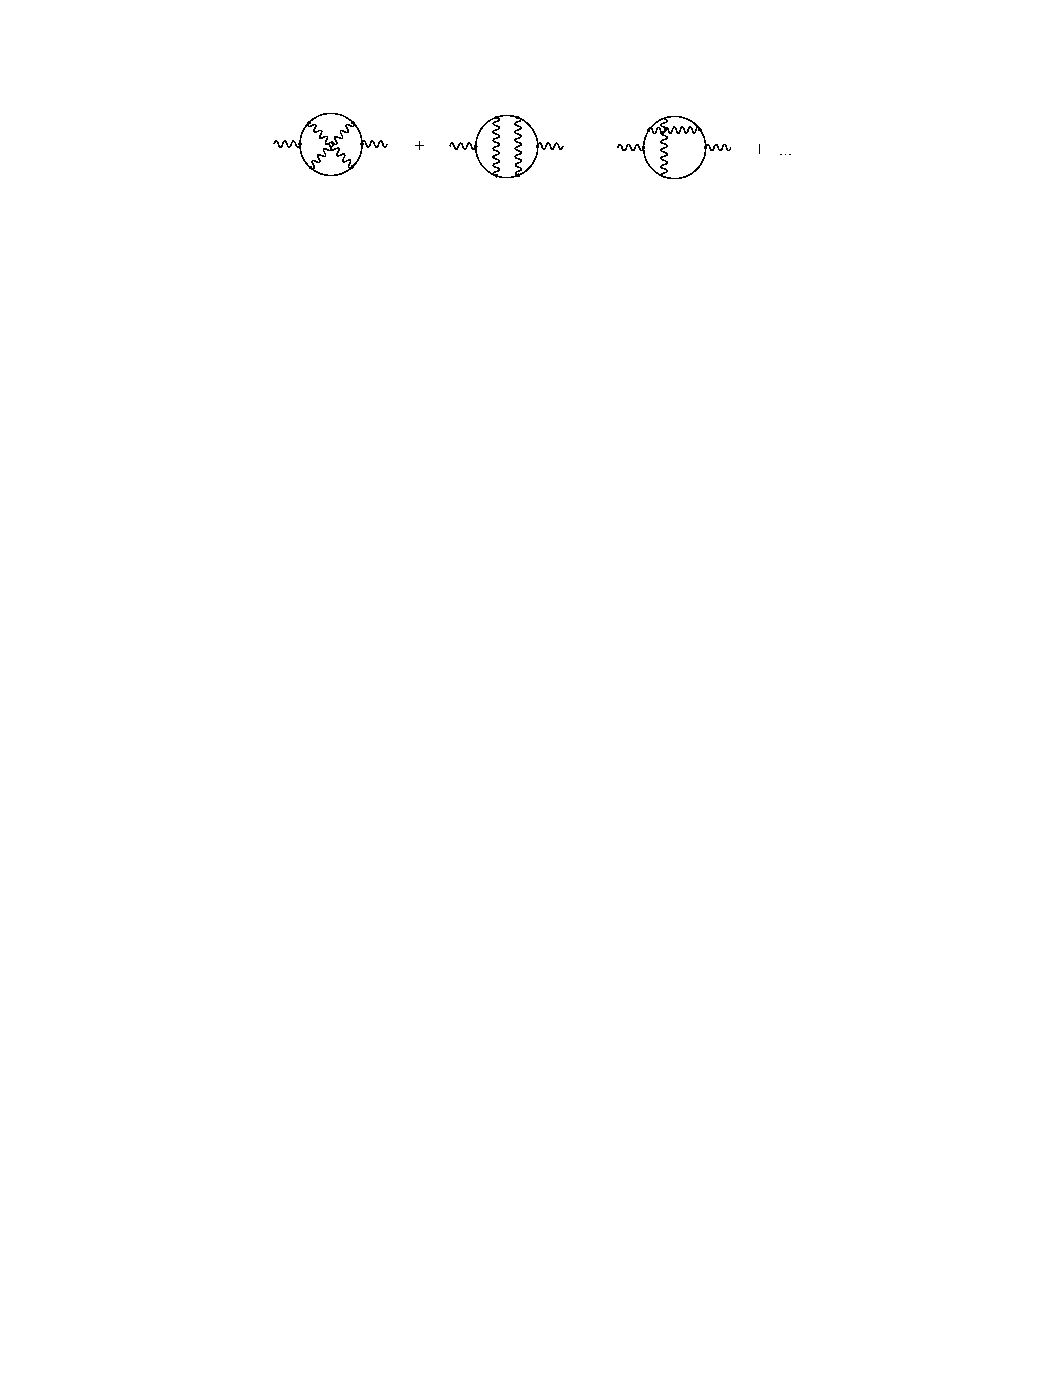
\includegraphics[width=1\textwidth]{BHSTW143loopphotonprop}
 \caption{Diagrams contributing to the three loop QED photon propagator.
 From \refref{BHSTW14}.
 }
 \label{BHSTW143loopphotonprop}
\end{figure}

This property is particularly interesting in view of the fact that it is
just this type of summation which in QED often leads to extensive
cancellations, and to final results which are substantially simpler than
intermediate ones (see, e.g., \refref{Cvit77b,BrDeKr96}). More recently, similar
cancellations have been found also for graviton amplitudes (see, e.g.,
\refref{BaBjVa09}).
Although this property of the worldline formalism is well-known, and has
been occasionally exploited\rf{rossch96a,rossch96b, SchSch96,BaRoSt06} (see also
\refref{FriGab12}) a systematic study of its implications is
presently still lacking.

In the spinor QED case (fermion lines and photon exchanges) closed-form
expressions for general $N$ could still be achieved using the worldline
super-\,formalism\rf{Schubert01}, however at the cost of introducing
additional multiple Grassmann integrals.

\item[2017-05-23 Predrag]
Huet, de Traubenberg, and Schubert\rf{HuTrSc17}
{\em Multiloop {Euler-\,Heisenberg Lagrangians, Schwinger} pair creation,
and the photon {S-matrix}}:
``Schwinger pair creation in a constant electric field, may possibly
provide a window to high loop orders; simple non-perturbative closed-form
expressions have been conjectured for the pair creation rate in the weak
field limit, for scalar QED in 1982 by Affleck, Alvarez, and
Manton\rf{AffAlMa82}, and for spinor QED by Lebedev and
Ritus\rf{LebRit84} in 1984. Using Borel analysis, these can be used to
obtain non-perturbative information on the on-shell renormalized N-photon
amplitudes at large N and low energy. This line of reasoning also leads
to a number of nontrivial predictions for the effective QED Lagrangian in
either four or two dimensions at any loop order, and preliminary results
of a calculation of the three-loop Euler--Heisenberg Lagrangian in two
dimensions are presented.''

Das, Frenkel and ,Schubert\rf{DaFrSc13}
{\em Infrared divergences, mass shell singularities and gauge dependence
of the dynamical fermion mass} \arXiv{1212.2057}:

Ahmadiniaz, Bashir and Schubert\rf{AhBaSc16}
{\em Multiphoton amplitudes and generalized {Landau-Khalatnikov-Fradkin}
transformation in scalar {QED}},  	\arXiv{1511.05087}:

Ahmad \etal\rf{AACKS17}
{\em Master formulas for the dressed scalar propagator in a constant field},
\arXiv{1612.02944}


\item[2017-05-23 Predrag]
Broadhurst and R. Delbourgo and D. Kreimer\rf{BrDeKr96}
{\em Unknotting the polarized vacuum of quenched {QED}}

\item[2017-05-23 Predrag]
Dirk Kreimer and
\HREF{https://arxiv.org/find/math-ph,math/1/au:+Yeats_K/0/1/0/all/0/1}
{Karen Yeats}\rf{KreYea08}
{\em Recursion and growth estimates in renormalizable quantum field theory}

Yeats\rf{Yeats17} {\em {A Combinatorial Perspective on Quantum Field Theory}}.
I have put a copy \HREF{http://ChaosBook.org/library/Yeats17.pdf}{here}.

\item[2016-08-20 Predrag]
Ki{\ss}ler and Kreimer\rf{KisKre16}
{Diagrammatic cancellations and the gauge dependence of {QED}}:
``
The perturbative expansion given in terms of Feynman graphs might be
rearranged in terms of meta graphs or subsectors with a maximum number of
cancellations implemented. An early attempt to construct gauge invariant
subsectors in QCD was given by Cvitanovi\'c \etal\rf{NPB81}.
''

Read also Kreimer\rf{Kreimer00}
{\em Knots and {Feynman} diagrams}.


\item[2017-05-23 Predrag]
Badger, Bjerrum-Bohr and Vanhove\rf{BaBjVa09}
{\em Simplicity in the structure of {QED} and gravity amplitudes}

\item[2017-05-23 Predrag]
Rosenfelder and Schreiber\rf{rossch96a,rossch96b},
\arXiv{nucl-th/9504002}, \arXiv{nucl-th/9504005}:

\item[2017-05-23 Predrag]
K. Barro-Bergfl\"odt, R. Rosenfelder and M. Stingl\rf{BaRoSt06} {\em
Variational worldline approximation for the relativistic two-body bound
state in a scalar model}, \arXiv{hep-ph/0601220}.

\item[2017-03-15 Predrag] Read
Fried\rf{Fried14}
{\em Modern Functional Quantum Field Theory: Summing Feynman Graphs}:
a simple, analytic, functional approach to non-perturbative QFT, using a
functional representation of Fradkin to explicitly
calculate relevant portions of the Schwinger Generating Functional (GF).
In QED, this corresponds to

\emph{summing all Feynman graphs representing virtual photon exchange}

between charged particles. It is then possible to
see, analytically, the cancellation of an infinite number of
perturbative, UV logarithmic divergences, leading to an approximate but
most reasonable statement of finite charge renormalization. A similar
treatment of QCD, with the addition of a long-overlooked but simple
rearrangement of the Schwinger GF which displays Manifest Gauge
Invariance, is then able to produce a simple, analytic derivation of
quark-binding potentials without any approximation of infinite quark
masses. A crucial improvement of previous QCD theory takes into account
the experimental fact that asymptotic quarks are always found in bound
state.

This book can be read online via \texttt{library.gatech.edu}


\item[2017-05-23 Predrag]
H.~M. Fried and Y. Gabellini\rf{FriGab12},
{\em On the Summation of Feynman Graphs}, \arXiv{1004.2202}.


\end{description}
